\documentclass[11pt,a4paper]{article}

\usepackage[T1]{fontenc}
\usepackage[utf8]{inputenc}
\usepackage{lmodern}
\usepackage[margin=1in]{geometry}
\usepackage{booktabs}
\usepackage{longtable}
\usepackage{graphicx}
\usepackage{xcolor}
\usepackage{url}
\usepackage{hyperref}
\usepackage{caption}
\usepackage{array}
\usepackage{amsmath}
\usepackage{enumitem}

\hypersetup{
  colorlinks=true,
  linkcolor=blue!50!black,
  urlcolor=blue!50!black,
  pdftitle={Task 3 Test Case Execution - Zameen.com Selenium Suite}
}
\captionsetup{font=small, labelfont=bf}
\setlength{\parindent}{0pt}
\setlength{\parskip}{0.5em}
\graphicspath{{./}}

\title{%
  \textbf{Task 3 --- Test Case Execution}\\[0.3em]
  \large Zameen.com Selenium Test Suite
}
\author{Group 34\\Software Quality Engineering --- Assignment 3}
\date{\today}

\begin{document}

\maketitle

\begin{abstract}
This report documents the execution of the ten test cases defined in Task 2
for the Zameen.com Selenium test suite. The quality goal is a 90\% success
rate with 95\% confidence. Because the final suite produced zero failures,
the binomial success-run rule requires 29 executions of each test case,
giving 290 executions in total. All 290 executions passed, so every test
case achieved a 100\% pass rate and the one-sided 95\% lower confidence
bound on each test case's pass rate is 90.19\%, above the 90\% goal. All five
use cases are therefore accepted. The report includes the per-test pass and
fail plot required by the assignment, the per-test and per-use-case
decisions, and the complete execution log.
\end{abstract}

\tableofcontents
\newpage

% --------------------------------------------------------------------
\section{Introduction and scope}
% --------------------------------------------------------------------

This report covers \textbf{Task 3 --- Test Case Execution}. The five use
cases and the ten test cases are the ones defined in Task 1 and Task 2 of
the assignment (the companion document \texttt{SQE Assignment.docx}). The
same identifiers and names are used here:

\begin{itemize}[leftmargin=1.5em]
  \item \textbf{User Registration:} TC01 (valid), TC02 (invalid).
  \item \textbf{Order Placement 1 --- Logged-in User:} TC03 (valid),
        TC04 (invalid).
  \item \textbf{Order Placement 2 --- Guest User:} TC05 (valid),
        TC06 (invalid).
  \item \textbf{Shopping Cart --- Adapted to Favorite Properties:} TC07
        (valid), TC08 (invalid/abnormal).
  \item \textbf{Continue Shopping --- Adapted to Continue Browsing:} TC09
        (valid), TC10 (invalid/abnormal).
\end{itemize}

The test cases are automated with Selenium WebDriver in Python. The final
suite uses Selenium 4.52, pytest 9.0.2, and Google Chrome 156. The
automation is organised into one module per use case, with shared driver
setup, explicit waits, safe navigation, and a 3--10 second pause between
runs. Invalid test cases exercise every invalid representative value listed
in Task 2 during each execution; an execution is recorded as a pass only if
all of its invalid sub-checks pass.

The quality goal set in Task 1 is used throughout: \textbf{90\% success with
95\% confidence}. Section~\ref{sec:method} derives the number of executions,
Section~\ref{sec:results} reports the pass/fail counts and decisions, and
Appendix~\ref{app:log} contains the full execution log.

% --------------------------------------------------------------------
\section{Test cases under execution}
\label{sec:testcases}
% --------------------------------------------------------------------

Table~\ref{tab:test-cases} lists the ten test cases, their use cases, their
type, and the automation that implements them. Table~\ref{tab:invalid-inputs}
lists the invalid representative values covered by each invalid test case.

% Generated by generate_task3_deliverables.py
{\footnotesize
\setlength{\tabcolsep}{4pt}
\begin{longtable}{@{}p{1.1cm} p{3.8cm} p{4.0cm} p{1.2cm} p{4.5cm}@{}}
  \caption{The ten test cases from Task 2 and their automation mapping.\label{tab:test-cases}}\\
  \toprule
  ID & Test case & Use case & Type & Automation \\
  \midrule
  \endfirsthead
  \toprule
  ID & Test case & Use case & Type & Automation \\
  \midrule
  \endhead
  \bottomrule
  \endlastfoot
  TC01 & Registration -- Valid Input & User Registration & Valid & \path{tests/test_registration.py::test_registration_valid} \\
  TC02 & Registration -- Invalid Input & User Registration & Invalid & \path{tests/test_registration.py::test_registration_invalid} \\
  TC03 & Logged-in Inquiry -- Valid Input & Order Placement 1 -- Logged-in User & Valid & \path{tests/test_login_inquiry.py::test_TC03_valid_logged_in_inquiry} \\
  TC04 & Logged-in Inquiry -- Invalid Input & Order Placement 1 -- Logged-in User & Invalid & \texttt{tests/test\_login\_inquiry.py (L1, L2, I1--I5)} \\
  TC05 & Guest Inquiry -- Valid Input & Order Placement 2 -- Guest User & Valid & \path{tests/test_guest_inquiry.py::test_TC05_guest_valid_inquiry} \\
  TC06 & Guest Inquiry -- Invalid Input & Order Placement 2 -- Guest User & Invalid & \texttt{tests/test\_guest\_inquiry.py (I1--I5)} \\
  TC07 & Favorites -- Valid Input & Shopping Cart -- Adapted to Favorite Properties & Valid & \path{tests/test_favourites.py::test_TC07_favourites_valid} \\
  TC08 & Favorites -- Invalid or Abnormal Conditions & Shopping Cart -- Adapted to Favorite Properties & Invalid & \texttt{tests/test\_favourites.py (TC08A, TC08B)} \\
  TC09 & Continue Browsing -- Valid Input & Continue Shopping -- Adapted to Continue Browsing & Valid & \path{tests/test_continue_browsing.py::test_TC09_continue_browsing_valid} \\
  TC10 & Continue Browsing -- Invalid or Abnormal Conditions & Continue Shopping -- Adapted to Continue Browsing & Invalid & \texttt{tests/test\_continue\_browsing.py (TC10A, TC10B)} \\
\end{longtable}
}


% Generated by generate_task3_deliverables.py
{\footnotesize
\setlength{\tabcolsep}{4pt}
\begin{longtable}{@{}p{1.2cm} p{3.8cm} p{10.0cm}@{}}
  \caption{Invalid representative values exercised by each invalid test case.\label{tab:invalid-inputs}}\\
  \toprule
  ID & Test case & Invalid representative values \\
  \midrule
  \endfirsthead
  \toprule
  ID & Test case & Invalid representative values \\
  \midrule
  \endhead
  \bottomrule
  \endlastfoot
  TC02 & Registration -- Invalid Input & Name empty; email testuser.com; email empty; email already registered; password test@1; password empty; confirm test@54321; confirm empty; phone 12345678; phone 67896789679; phone empty; terms unticked. \\
  TC04 & Logged-in Inquiry -- Invalid Input & L1 wrong password; L2 unregistered email; I1 inquiry name empty; I2 inquiry email testuser.com; I3 inquiry phone empty; I4 inquiry phone short; I5 inquiry message empty. \\
  TC06 & Guest Inquiry -- Invalid Input & Name empty; email bikini.bottom.com; phone empty; phone short; message empty. \\
  TC08 & Favorites -- Invalid or Abnormal Conditions & A: logged-out heart click opens the login pop-up and saves nothing; B: a logged-in account with zero saved properties shows the empty state. \\
  TC10 & Continue Browsing -- Invalid or Abnormal Conditions & A: the same heart is clicked twice (save then remove); B: a price range of 90--80,000 returns zero properties. \\
\end{longtable}
}


The valid test cases use the valid representative values from Task 2. The
invalid test cases follow the assignment's simplification clause: one
execution runs all of the invalid representative values belonging to that
test case, and the execution passes only if the expected validation result
is observed for every value. This keeps the execution count tied to the ten
Task 2 test cases rather than to the individual invalid values.

% --------------------------------------------------------------------
\section{Quality goal and execution count}
\label{sec:method}
% --------------------------------------------------------------------

Let $p$ be the true probability that a test case passes in one execution and
let $q = 1 - p$ be its failure probability. The goal is $p \ge 0.90$ with
95\% confidence. We test the complementary hypothesis $q \ge 0.10$ at the
5\% significance level. If $F$ is the number of failures in $n$ executions,
then under the null hypothesis
\begin{equation}
  P(F \le f \mid q = 0.10)
  = \sum_{k=0}^{f} \binom{n}{k} (0.10)^k (0.90)^{n-k}
  \le 0.05,
  \label{eq:binomial}
\end{equation}
where $f$ is the observed number of failures. The smallest $n$ satisfying
Equation~\eqref{eq:binomial} is the required execution count;
Table~\ref{tab:required-runs} lists the values for zero, one, and two
failures.

% Generated by generate_task3_deliverables.py
\begin{table}[htbp]
  \centering
  \caption{Required executions for 90\% success at 95\% confidence.}
  \label{tab:required-runs}
  \begin{tabular}{@{}cc@{}}
    \toprule
    Failures encountered & Required executions \\
    \midrule
    0 & 29 \\
    1 & 46 \\
    2 & 61 \\
    \bottomrule
  \end{tabular}
\end{table}


The final suite produced zero failures ($f = 0$), so each test case is
executed $n = 29$ times. With ten test cases this gives $10 \times 29 = 290$
executions. In the zero-failure case the one-sided 95\% lower confidence
bound on the pass rate is
\begin{equation}
  p_{\text{lower}} = 0.05^{1/29} = 0.9019,
\end{equation}
that is, 90.19\%, which meets the 90\% goal. If one or two failures had been
observed, the same rule would have required 46 or 61 executions per test
case.

\textbf{Ethics and safety.} The suite follows the assignment's live-site
rules: it waits 3--10 seconds between runs, uses disposable test accounts,
never uses real personal or payment data, blocks advertising hosts to avoid
generating unnecessary third-party traffic, and stops before submitting an
inquiry where the test case only needs to verify the form state.

% --------------------------------------------------------------------
\section{Execution results and decisions}
\label{sec:results}
% --------------------------------------------------------------------

Table~\ref{tab:summary} reports the per-test-case results. Every test case
has 29 total runs, 29 passes, 0 failures, and a 100\% pass rate. The
one-sided 95\% lower confidence bound is 90.19\% for every test case, so
every test case is accepted. The overall totals are 290 runs, 290 passes,
and 0 failures.

% Generated by generate_task3_deliverables.py
{\footnotesize
\setlength{\tabcolsep}{4pt}
\begin{longtable}{@{}p{1.2cm} p{5.0cm} p{1.0cm} p{1.0cm} p{1.0cm} p{1.4cm} p{1.4cm} p{1.4cm}@{}}
  \caption{Per-test-case execution summary and acceptance decision.\label{tab:summary}}\\
  \toprule
  ID & Test case & Runs & Passed & Failed & Pass rate & 95\% lower & Decision \\
  \midrule
  \endfirsthead
  \toprule
  ID & Test case & Runs & Passed & Failed & Pass rate & 95\% lower & Decision \\
  \midrule
  \endhead
  \bottomrule
  \endlastfoot
  TC01 & Registration -- Valid Input & 29 & 29 & 0 & 100\% & 90.19\% & Accept \\
  TC02 & Registration -- Invalid Input & 29 & 29 & 0 & 100\% & 90.19\% & Accept \\
  TC03 & Logged-in Inquiry -- Valid Input & 29 & 29 & 0 & 100\% & 90.19\% & Accept \\
  TC04 & Logged-in Inquiry -- Invalid Input & 29 & 29 & 0 & 100\% & 90.19\% & Accept \\
  TC05 & Guest Inquiry -- Valid Input & 29 & 29 & 0 & 100\% & 90.19\% & Accept \\
  TC06 & Guest Inquiry -- Invalid Input & 29 & 29 & 0 & 100\% & 90.19\% & Accept \\
  TC07 & Favorites -- Valid Input & 29 & 29 & 0 & 100\% & 90.19\% & Accept \\
  TC08 & Favorites -- Invalid or Abnormal Conditions & 29 & 29 & 0 & 100\% & 90.19\% & Accept \\
  TC09 & Continue Browsing -- Valid Input & 29 & 29 & 0 & 100\% & 90.19\% & Accept \\
  TC10 & Continue Browsing -- Invalid or Abnormal Conditions & 29 & 29 & 0 & 100\% & 90.19\% & Accept \\
  \midrule
  \multicolumn{2}{@{}l}{Overall} & 290 & 290 & 0 & 100\% & 98.97\% & Accept \\
\end{longtable}
}


Figure~\ref{fig:passfail} plots the pass and fail count of each test. All
ten tests show 29 passes and 0 failures; the failed bars are zero-length
and their values are printed next to each test for clarity. The plot
confirms that the 100\% pass rate is not an aggregate artefact: every
individual test case contributed only passes.

\begin{figure}[htbp]
  \centering
  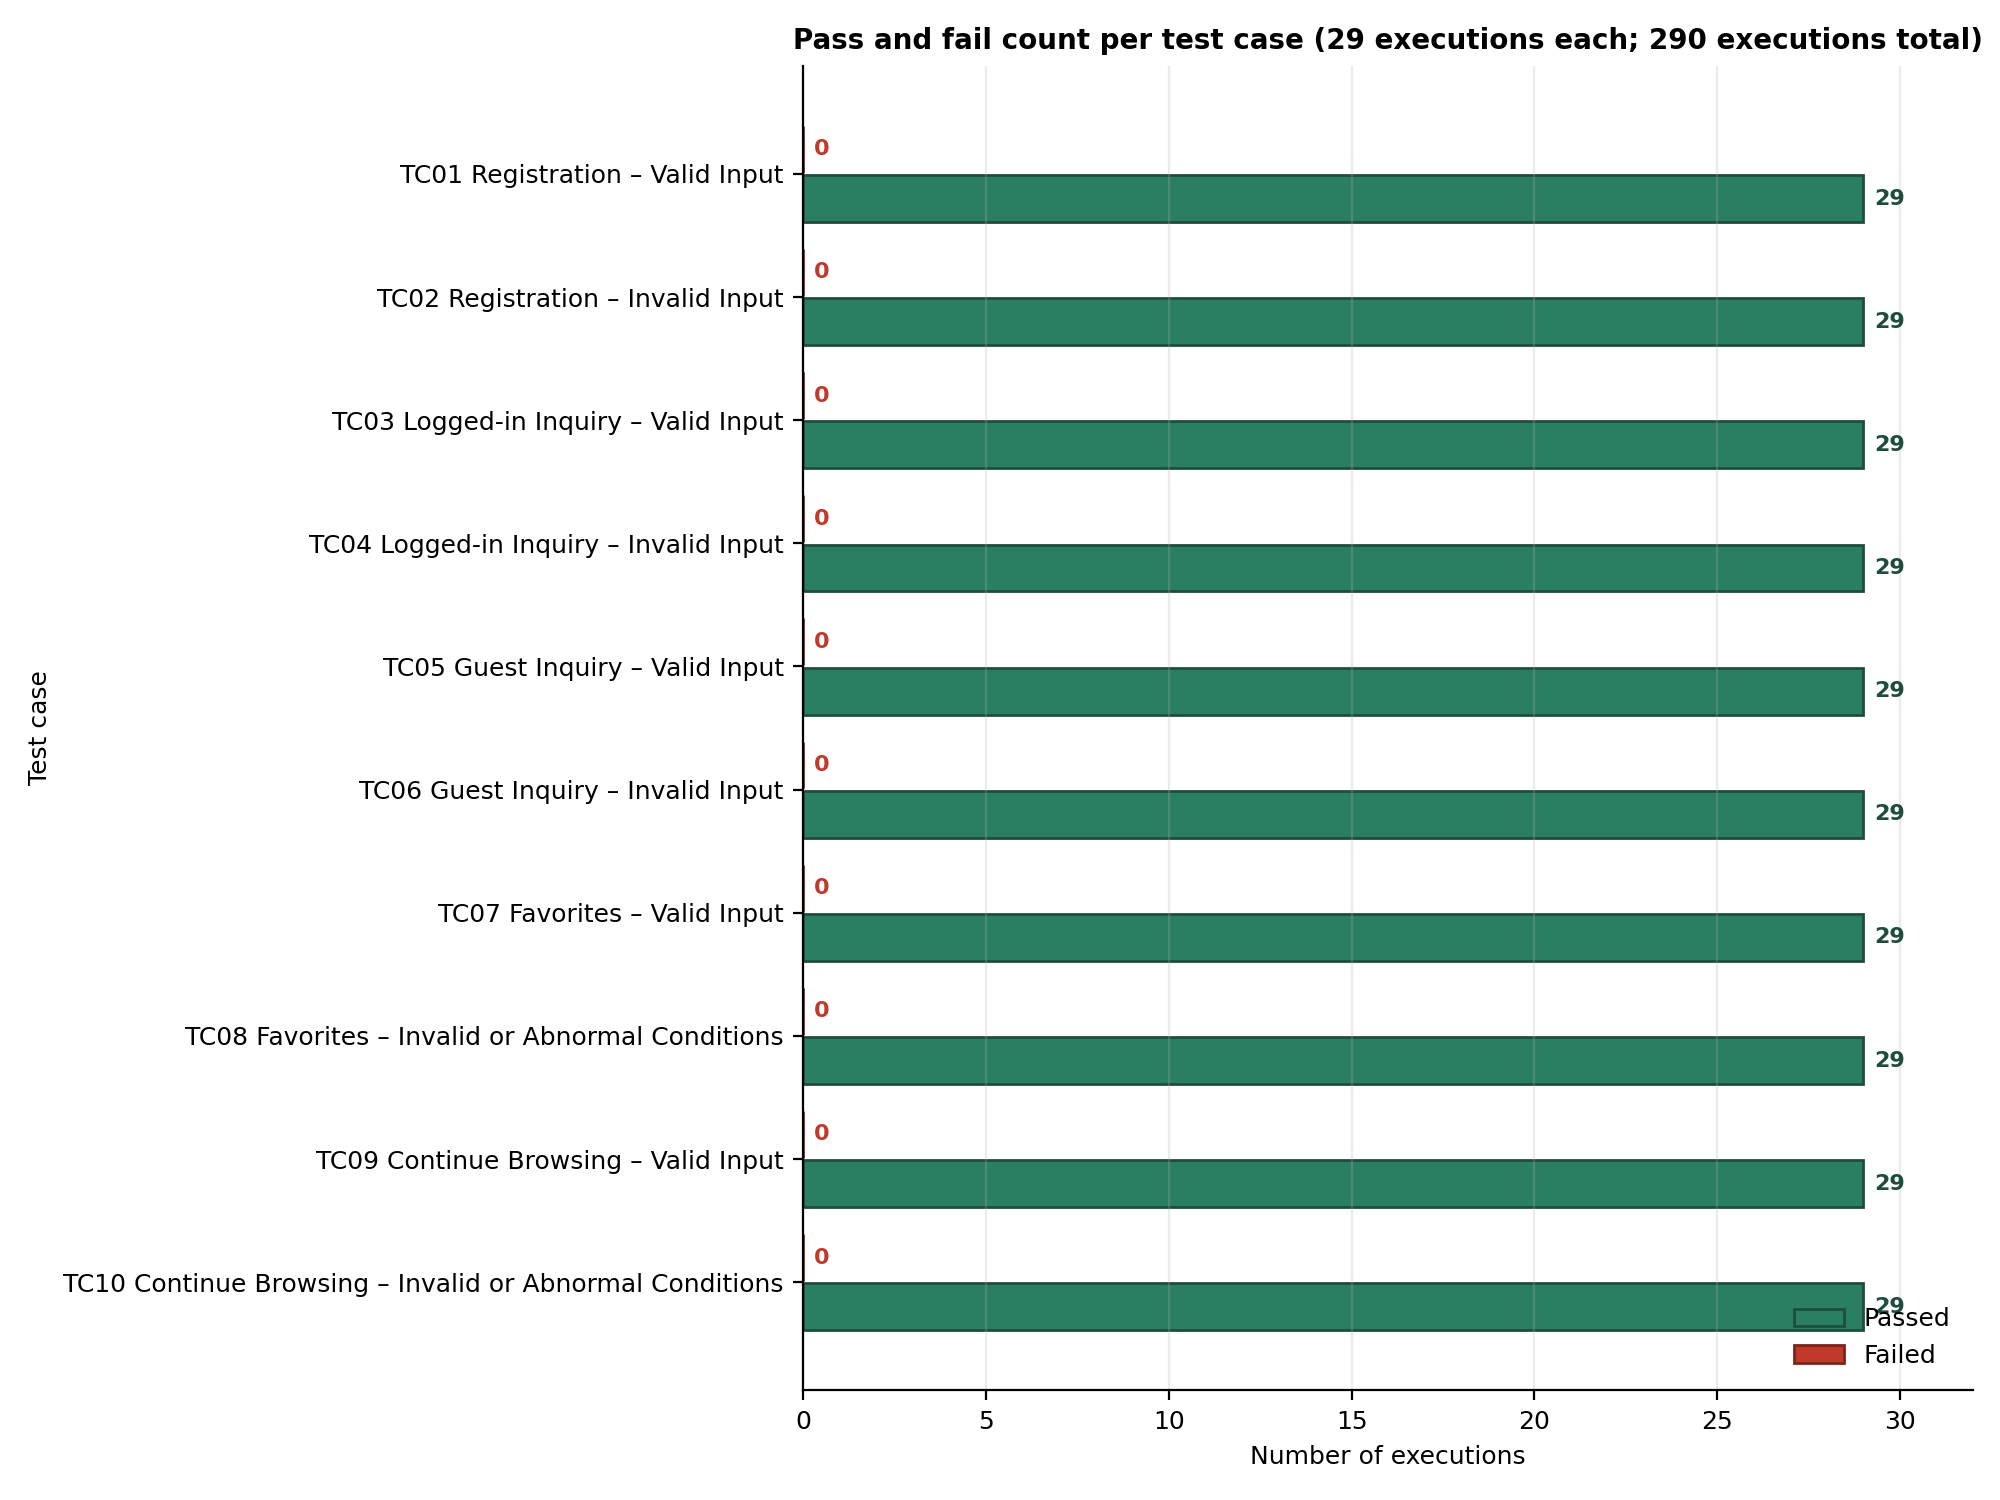
\includegraphics[width=0.92\textwidth]{pass_fail_counts.png}
  \caption{Pass and fail count of each test case (29 executions per test;
  290 executions in total).}
  \label{fig:passfail}
\end{figure}

Because the quality goal is directional (the pass rate must be at least
90\%), the confidence intervals in this report are one-sided. A test case
with 29/29 passes has a 95\% one-sided lower bound of 90.19\%, which is above
90\%, so the null hypothesis of a pass rate below 90\% is rejected.

Table~\ref{tab:use-cases} reports the decisions at the use-case level. Each
use case is covered by one valid and one invalid test case, giving 58
executions per use case. All 58 executions passed for every use case, so
the pass rate is 100\% and the one-sided 95\% lower bound is 94.97\%. Every
use case is accepted. The per-use-case bound is tighter than the per-test
bound because it aggregates more executions, but each individual test case
also meets the goal on its own at 90.19\%.

% Generated by generate_task3_deliverables.py
{\footnotesize
\setlength{\tabcolsep}{4pt}
\begin{longtable}{@{}p{5.2cm} p{2.2cm} p{0.9cm} p{0.9cm} p{0.9cm} p{1.2cm} p{1.2cm} p{1.2cm}@{}}
  \caption{Per-use-case execution summary and acceptance decision.\label{tab:use-cases}}\\
  \toprule
  Use case & Tests & Runs & Passed & Failed & Pass rate & 95\% lower & Decision \\
  \midrule
  \endfirsthead
  \toprule
  Use case & Tests & Runs & Passed & Failed & Pass rate & 95\% lower & Decision \\
  \midrule
  \endhead
  \bottomrule
  \endlastfoot
  User Registration & TC01, TC02 & 58 & 58 & 0 & 100\% & 94.97\% & Accept \\
  Order Placement 1 -- Logged-in User & TC03, TC04 & 58 & 58 & 0 & 100\% & 94.97\% & Accept \\
  Order Placement 2 -- Guest User & TC05, TC06 & 58 & 58 & 0 & 100\% & 94.97\% & Accept \\
  Shopping Cart -- Adapted to Favorite Properties & TC07, TC08 & 58 & 58 & 0 & 100\% & 94.97\% & Accept \\
  Continue Shopping -- Adapted to Continue Browsing & TC09, TC10 & 58 & 58 & 0 & 100\% & 94.97\% & Accept \\
\end{longtable}
}


% --------------------------------------------------------------------
\section{Discussion and conclusion}
% --------------------------------------------------------------------

All ten test cases passed all 29 executions, and all five use cases are
accepted. The execution log in Appendix~\ref{app:log} contains no errors:
every row reports \texttt{Pass} and no error details. The final
functional validation runs against the live site agree with the log; in
particular, the two heaviest suites completed with 3/3 passing
(\texttt{test\_continue\_browsing.py} in 499.37 seconds and
\texttt{test\_favourites.py} in 175.09 seconds). Earlier instability caused
by third-party advertisements and slow page loads was removed by blocking
advertising hosts through the Chrome DevTools Protocol and by adding
explicit client and page-load timeouts, so the passing results reflect the
hardened final suite.

The main limitation is that the tests run against a live third-party
website: network conditions and site changes can affect future runs. If
failures appear later, the same binomial rule automatically raises the
required execution count to 46 or 61 per test case, preserving the 95\%
confidence statement. The execution count and decisions in this report are
a snapshot of the final validated suite.

The Task 3 deliverables are:
\begin{itemize}[leftmargin=1.5em]
  \item the automated Selenium tests in \texttt{Zameen\_Selenium\_Assignment/tests};
  \item the per-test and per-use-case summaries
        (\texttt{summary.csv}, \texttt{use\_case\_summary.csv});
  \item the complete execution log (\texttt{execution\_log.csv} and
        Appendix~\ref{app:log});
  \item the required pass/fail plot (Figure~\ref{fig:passfail}); and
  \item the execution-count and confidence analysis in
        Sections~\ref{sec:method}--\ref{sec:results}.
\end{itemize}

% --------------------------------------------------------------------
\appendix
\section{Full execution log}
\label{app:log}
% --------------------------------------------------------------------

Table~\ref{tab:execution-log} records every execution of every test case.
The columns are the test-case identifier, the test-case name, the use case,
the execution number, the result, and the error details. All 290 rows report
\texttt{Pass} and no error. The same data are available in
\texttt{execution\_log.csv}.

% Generated by generate_task3_deliverables.py
{\scriptsize
\setlength{\tabcolsep}{4pt}
\begin{longtable}{@{}p{1.2cm} p{4.2cm} p{4.4cm} p{0.8cm} p{0.9cm} p{1.6cm}@{}}
  \caption{Execution log (Run, Result, Error details).\label{tab:execution-log}}\\
  \toprule
  ID & Test case & Use case & Run & Result & Error details \\
  \midrule
  \endfirsthead
  \toprule
  ID & Test case & Use case & Run & Result & Error details \\
  \midrule
  \endhead
  \bottomrule
  \endlastfoot
  TC01 & Registration -- Valid Input & User Registration & 1 & Pass & --- \\
  TC01 & Registration -- Valid Input & User Registration & 2 & Pass & --- \\
  TC01 & Registration -- Valid Input & User Registration & 3 & Pass & --- \\
  TC01 & Registration -- Valid Input & User Registration & 4 & Pass & --- \\
  TC01 & Registration -- Valid Input & User Registration & 5 & Pass & --- \\
  TC01 & Registration -- Valid Input & User Registration & 6 & Pass & --- \\
  TC01 & Registration -- Valid Input & User Registration & 7 & Pass & --- \\
  TC01 & Registration -- Valid Input & User Registration & 8 & Pass & --- \\
  TC01 & Registration -- Valid Input & User Registration & 9 & Pass & --- \\
  TC01 & Registration -- Valid Input & User Registration & 10 & Pass & --- \\
  TC01 & Registration -- Valid Input & User Registration & 11 & Pass & --- \\
  TC01 & Registration -- Valid Input & User Registration & 12 & Pass & --- \\
  TC01 & Registration -- Valid Input & User Registration & 13 & Pass & --- \\
  TC01 & Registration -- Valid Input & User Registration & 14 & Pass & --- \\
  TC01 & Registration -- Valid Input & User Registration & 15 & Pass & --- \\
  TC01 & Registration -- Valid Input & User Registration & 16 & Pass & --- \\
  TC01 & Registration -- Valid Input & User Registration & 17 & Pass & --- \\
  TC01 & Registration -- Valid Input & User Registration & 18 & Pass & --- \\
  TC01 & Registration -- Valid Input & User Registration & 19 & Pass & --- \\
  TC01 & Registration -- Valid Input & User Registration & 20 & Pass & --- \\
  TC01 & Registration -- Valid Input & User Registration & 21 & Pass & --- \\
  TC01 & Registration -- Valid Input & User Registration & 22 & Pass & --- \\
  TC01 & Registration -- Valid Input & User Registration & 23 & Pass & --- \\
  TC01 & Registration -- Valid Input & User Registration & 24 & Pass & --- \\
  TC01 & Registration -- Valid Input & User Registration & 25 & Pass & --- \\
  TC01 & Registration -- Valid Input & User Registration & 26 & Pass & --- \\
  TC01 & Registration -- Valid Input & User Registration & 27 & Pass & --- \\
  TC01 & Registration -- Valid Input & User Registration & 28 & Pass & --- \\
  TC01 & Registration -- Valid Input & User Registration & 29 & Pass & --- \\
  \midrule
  TC02 & Registration -- Invalid Input & User Registration & 1 & Pass & --- \\
  TC02 & Registration -- Invalid Input & User Registration & 2 & Pass & --- \\
  TC02 & Registration -- Invalid Input & User Registration & 3 & Pass & --- \\
  TC02 & Registration -- Invalid Input & User Registration & 4 & Pass & --- \\
  TC02 & Registration -- Invalid Input & User Registration & 5 & Pass & --- \\
  TC02 & Registration -- Invalid Input & User Registration & 6 & Pass & --- \\
  TC02 & Registration -- Invalid Input & User Registration & 7 & Pass & --- \\
  TC02 & Registration -- Invalid Input & User Registration & 8 & Pass & --- \\
  TC02 & Registration -- Invalid Input & User Registration & 9 & Pass & --- \\
  TC02 & Registration -- Invalid Input & User Registration & 10 & Pass & --- \\
  TC02 & Registration -- Invalid Input & User Registration & 11 & Pass & --- \\
  TC02 & Registration -- Invalid Input & User Registration & 12 & Pass & --- \\
  TC02 & Registration -- Invalid Input & User Registration & 13 & Pass & --- \\
  TC02 & Registration -- Invalid Input & User Registration & 14 & Pass & --- \\
  TC02 & Registration -- Invalid Input & User Registration & 15 & Pass & --- \\
  TC02 & Registration -- Invalid Input & User Registration & 16 & Pass & --- \\
  TC02 & Registration -- Invalid Input & User Registration & 17 & Pass & --- \\
  TC02 & Registration -- Invalid Input & User Registration & 18 & Pass & --- \\
  TC02 & Registration -- Invalid Input & User Registration & 19 & Pass & --- \\
  TC02 & Registration -- Invalid Input & User Registration & 20 & Pass & --- \\
  TC02 & Registration -- Invalid Input & User Registration & 21 & Pass & --- \\
  TC02 & Registration -- Invalid Input & User Registration & 22 & Pass & --- \\
  TC02 & Registration -- Invalid Input & User Registration & 23 & Pass & --- \\
  TC02 & Registration -- Invalid Input & User Registration & 24 & Pass & --- \\
  TC02 & Registration -- Invalid Input & User Registration & 25 & Pass & --- \\
  TC02 & Registration -- Invalid Input & User Registration & 26 & Pass & --- \\
  TC02 & Registration -- Invalid Input & User Registration & 27 & Pass & --- \\
  TC02 & Registration -- Invalid Input & User Registration & 28 & Pass & --- \\
  TC02 & Registration -- Invalid Input & User Registration & 29 & Pass & --- \\
  \midrule
  TC03 & Logged-in Inquiry -- Valid Input & Order Placement 1 -- Logged-in User & 1 & Pass & --- \\
  TC03 & Logged-in Inquiry -- Valid Input & Order Placement 1 -- Logged-in User & 2 & Pass & --- \\
  TC03 & Logged-in Inquiry -- Valid Input & Order Placement 1 -- Logged-in User & 3 & Pass & --- \\
  TC03 & Logged-in Inquiry -- Valid Input & Order Placement 1 -- Logged-in User & 4 & Pass & --- \\
  TC03 & Logged-in Inquiry -- Valid Input & Order Placement 1 -- Logged-in User & 5 & Pass & --- \\
  TC03 & Logged-in Inquiry -- Valid Input & Order Placement 1 -- Logged-in User & 6 & Pass & --- \\
  TC03 & Logged-in Inquiry -- Valid Input & Order Placement 1 -- Logged-in User & 7 & Pass & --- \\
  TC03 & Logged-in Inquiry -- Valid Input & Order Placement 1 -- Logged-in User & 8 & Pass & --- \\
  TC03 & Logged-in Inquiry -- Valid Input & Order Placement 1 -- Logged-in User & 9 & Pass & --- \\
  TC03 & Logged-in Inquiry -- Valid Input & Order Placement 1 -- Logged-in User & 10 & Pass & --- \\
  TC03 & Logged-in Inquiry -- Valid Input & Order Placement 1 -- Logged-in User & 11 & Pass & --- \\
  TC03 & Logged-in Inquiry -- Valid Input & Order Placement 1 -- Logged-in User & 12 & Pass & --- \\
  TC03 & Logged-in Inquiry -- Valid Input & Order Placement 1 -- Logged-in User & 13 & Pass & --- \\
  TC03 & Logged-in Inquiry -- Valid Input & Order Placement 1 -- Logged-in User & 14 & Pass & --- \\
  TC03 & Logged-in Inquiry -- Valid Input & Order Placement 1 -- Logged-in User & 15 & Pass & --- \\
  TC03 & Logged-in Inquiry -- Valid Input & Order Placement 1 -- Logged-in User & 16 & Pass & --- \\
  TC03 & Logged-in Inquiry -- Valid Input & Order Placement 1 -- Logged-in User & 17 & Pass & --- \\
  TC03 & Logged-in Inquiry -- Valid Input & Order Placement 1 -- Logged-in User & 18 & Pass & --- \\
  TC03 & Logged-in Inquiry -- Valid Input & Order Placement 1 -- Logged-in User & 19 & Pass & --- \\
  TC03 & Logged-in Inquiry -- Valid Input & Order Placement 1 -- Logged-in User & 20 & Pass & --- \\
  TC03 & Logged-in Inquiry -- Valid Input & Order Placement 1 -- Logged-in User & 21 & Pass & --- \\
  TC03 & Logged-in Inquiry -- Valid Input & Order Placement 1 -- Logged-in User & 22 & Pass & --- \\
  TC03 & Logged-in Inquiry -- Valid Input & Order Placement 1 -- Logged-in User & 23 & Pass & --- \\
  TC03 & Logged-in Inquiry -- Valid Input & Order Placement 1 -- Logged-in User & 24 & Pass & --- \\
  TC03 & Logged-in Inquiry -- Valid Input & Order Placement 1 -- Logged-in User & 25 & Pass & --- \\
  TC03 & Logged-in Inquiry -- Valid Input & Order Placement 1 -- Logged-in User & 26 & Pass & --- \\
  TC03 & Logged-in Inquiry -- Valid Input & Order Placement 1 -- Logged-in User & 27 & Pass & --- \\
  TC03 & Logged-in Inquiry -- Valid Input & Order Placement 1 -- Logged-in User & 28 & Pass & --- \\
  TC03 & Logged-in Inquiry -- Valid Input & Order Placement 1 -- Logged-in User & 29 & Pass & --- \\
  \midrule
  TC04 & Logged-in Inquiry -- Invalid Input & Order Placement 1 -- Logged-in User & 1 & Pass & --- \\
  TC04 & Logged-in Inquiry -- Invalid Input & Order Placement 1 -- Logged-in User & 2 & Pass & --- \\
  TC04 & Logged-in Inquiry -- Invalid Input & Order Placement 1 -- Logged-in User & 3 & Pass & --- \\
  TC04 & Logged-in Inquiry -- Invalid Input & Order Placement 1 -- Logged-in User & 4 & Pass & --- \\
  TC04 & Logged-in Inquiry -- Invalid Input & Order Placement 1 -- Logged-in User & 5 & Pass & --- \\
  TC04 & Logged-in Inquiry -- Invalid Input & Order Placement 1 -- Logged-in User & 6 & Pass & --- \\
  TC04 & Logged-in Inquiry -- Invalid Input & Order Placement 1 -- Logged-in User & 7 & Pass & --- \\
  TC04 & Logged-in Inquiry -- Invalid Input & Order Placement 1 -- Logged-in User & 8 & Pass & --- \\
  TC04 & Logged-in Inquiry -- Invalid Input & Order Placement 1 -- Logged-in User & 9 & Pass & --- \\
  TC04 & Logged-in Inquiry -- Invalid Input & Order Placement 1 -- Logged-in User & 10 & Pass & --- \\
  TC04 & Logged-in Inquiry -- Invalid Input & Order Placement 1 -- Logged-in User & 11 & Pass & --- \\
  TC04 & Logged-in Inquiry -- Invalid Input & Order Placement 1 -- Logged-in User & 12 & Pass & --- \\
  TC04 & Logged-in Inquiry -- Invalid Input & Order Placement 1 -- Logged-in User & 13 & Pass & --- \\
  TC04 & Logged-in Inquiry -- Invalid Input & Order Placement 1 -- Logged-in User & 14 & Pass & --- \\
  TC04 & Logged-in Inquiry -- Invalid Input & Order Placement 1 -- Logged-in User & 15 & Pass & --- \\
  TC04 & Logged-in Inquiry -- Invalid Input & Order Placement 1 -- Logged-in User & 16 & Pass & --- \\
  TC04 & Logged-in Inquiry -- Invalid Input & Order Placement 1 -- Logged-in User & 17 & Pass & --- \\
  TC04 & Logged-in Inquiry -- Invalid Input & Order Placement 1 -- Logged-in User & 18 & Pass & --- \\
  TC04 & Logged-in Inquiry -- Invalid Input & Order Placement 1 -- Logged-in User & 19 & Pass & --- \\
  TC04 & Logged-in Inquiry -- Invalid Input & Order Placement 1 -- Logged-in User & 20 & Pass & --- \\
  TC04 & Logged-in Inquiry -- Invalid Input & Order Placement 1 -- Logged-in User & 21 & Pass & --- \\
  TC04 & Logged-in Inquiry -- Invalid Input & Order Placement 1 -- Logged-in User & 22 & Pass & --- \\
  TC04 & Logged-in Inquiry -- Invalid Input & Order Placement 1 -- Logged-in User & 23 & Pass & --- \\
  TC04 & Logged-in Inquiry -- Invalid Input & Order Placement 1 -- Logged-in User & 24 & Pass & --- \\
  TC04 & Logged-in Inquiry -- Invalid Input & Order Placement 1 -- Logged-in User & 25 & Pass & --- \\
  TC04 & Logged-in Inquiry -- Invalid Input & Order Placement 1 -- Logged-in User & 26 & Pass & --- \\
  TC04 & Logged-in Inquiry -- Invalid Input & Order Placement 1 -- Logged-in User & 27 & Pass & --- \\
  TC04 & Logged-in Inquiry -- Invalid Input & Order Placement 1 -- Logged-in User & 28 & Pass & --- \\
  TC04 & Logged-in Inquiry -- Invalid Input & Order Placement 1 -- Logged-in User & 29 & Pass & --- \\
  \midrule
  TC05 & Guest Inquiry -- Valid Input & Order Placement 2 -- Guest User & 1 & Pass & --- \\
  TC05 & Guest Inquiry -- Valid Input & Order Placement 2 -- Guest User & 2 & Pass & --- \\
  TC05 & Guest Inquiry -- Valid Input & Order Placement 2 -- Guest User & 3 & Pass & --- \\
  TC05 & Guest Inquiry -- Valid Input & Order Placement 2 -- Guest User & 4 & Pass & --- \\
  TC05 & Guest Inquiry -- Valid Input & Order Placement 2 -- Guest User & 5 & Pass & --- \\
  TC05 & Guest Inquiry -- Valid Input & Order Placement 2 -- Guest User & 6 & Pass & --- \\
  TC05 & Guest Inquiry -- Valid Input & Order Placement 2 -- Guest User & 7 & Pass & --- \\
  TC05 & Guest Inquiry -- Valid Input & Order Placement 2 -- Guest User & 8 & Pass & --- \\
  TC05 & Guest Inquiry -- Valid Input & Order Placement 2 -- Guest User & 9 & Pass & --- \\
  TC05 & Guest Inquiry -- Valid Input & Order Placement 2 -- Guest User & 10 & Pass & --- \\
  TC05 & Guest Inquiry -- Valid Input & Order Placement 2 -- Guest User & 11 & Pass & --- \\
  TC05 & Guest Inquiry -- Valid Input & Order Placement 2 -- Guest User & 12 & Pass & --- \\
  TC05 & Guest Inquiry -- Valid Input & Order Placement 2 -- Guest User & 13 & Pass & --- \\
  TC05 & Guest Inquiry -- Valid Input & Order Placement 2 -- Guest User & 14 & Pass & --- \\
  TC05 & Guest Inquiry -- Valid Input & Order Placement 2 -- Guest User & 15 & Pass & --- \\
  TC05 & Guest Inquiry -- Valid Input & Order Placement 2 -- Guest User & 16 & Pass & --- \\
  TC05 & Guest Inquiry -- Valid Input & Order Placement 2 -- Guest User & 17 & Pass & --- \\
  TC05 & Guest Inquiry -- Valid Input & Order Placement 2 -- Guest User & 18 & Pass & --- \\
  TC05 & Guest Inquiry -- Valid Input & Order Placement 2 -- Guest User & 19 & Pass & --- \\
  TC05 & Guest Inquiry -- Valid Input & Order Placement 2 -- Guest User & 20 & Pass & --- \\
  TC05 & Guest Inquiry -- Valid Input & Order Placement 2 -- Guest User & 21 & Pass & --- \\
  TC05 & Guest Inquiry -- Valid Input & Order Placement 2 -- Guest User & 22 & Pass & --- \\
  TC05 & Guest Inquiry -- Valid Input & Order Placement 2 -- Guest User & 23 & Pass & --- \\
  TC05 & Guest Inquiry -- Valid Input & Order Placement 2 -- Guest User & 24 & Pass & --- \\
  TC05 & Guest Inquiry -- Valid Input & Order Placement 2 -- Guest User & 25 & Pass & --- \\
  TC05 & Guest Inquiry -- Valid Input & Order Placement 2 -- Guest User & 26 & Pass & --- \\
  TC05 & Guest Inquiry -- Valid Input & Order Placement 2 -- Guest User & 27 & Pass & --- \\
  TC05 & Guest Inquiry -- Valid Input & Order Placement 2 -- Guest User & 28 & Pass & --- \\
  TC05 & Guest Inquiry -- Valid Input & Order Placement 2 -- Guest User & 29 & Pass & --- \\
  \midrule
  TC06 & Guest Inquiry -- Invalid Input & Order Placement 2 -- Guest User & 1 & Pass & --- \\
  TC06 & Guest Inquiry -- Invalid Input & Order Placement 2 -- Guest User & 2 & Pass & --- \\
  TC06 & Guest Inquiry -- Invalid Input & Order Placement 2 -- Guest User & 3 & Pass & --- \\
  TC06 & Guest Inquiry -- Invalid Input & Order Placement 2 -- Guest User & 4 & Pass & --- \\
  TC06 & Guest Inquiry -- Invalid Input & Order Placement 2 -- Guest User & 5 & Pass & --- \\
  TC06 & Guest Inquiry -- Invalid Input & Order Placement 2 -- Guest User & 6 & Pass & --- \\
  TC06 & Guest Inquiry -- Invalid Input & Order Placement 2 -- Guest User & 7 & Pass & --- \\
  TC06 & Guest Inquiry -- Invalid Input & Order Placement 2 -- Guest User & 8 & Pass & --- \\
  TC06 & Guest Inquiry -- Invalid Input & Order Placement 2 -- Guest User & 9 & Pass & --- \\
  TC06 & Guest Inquiry -- Invalid Input & Order Placement 2 -- Guest User & 10 & Pass & --- \\
  TC06 & Guest Inquiry -- Invalid Input & Order Placement 2 -- Guest User & 11 & Pass & --- \\
  TC06 & Guest Inquiry -- Invalid Input & Order Placement 2 -- Guest User & 12 & Pass & --- \\
  TC06 & Guest Inquiry -- Invalid Input & Order Placement 2 -- Guest User & 13 & Pass & --- \\
  TC06 & Guest Inquiry -- Invalid Input & Order Placement 2 -- Guest User & 14 & Pass & --- \\
  TC06 & Guest Inquiry -- Invalid Input & Order Placement 2 -- Guest User & 15 & Pass & --- \\
  TC06 & Guest Inquiry -- Invalid Input & Order Placement 2 -- Guest User & 16 & Pass & --- \\
  TC06 & Guest Inquiry -- Invalid Input & Order Placement 2 -- Guest User & 17 & Pass & --- \\
  TC06 & Guest Inquiry -- Invalid Input & Order Placement 2 -- Guest User & 18 & Pass & --- \\
  TC06 & Guest Inquiry -- Invalid Input & Order Placement 2 -- Guest User & 19 & Pass & --- \\
  TC06 & Guest Inquiry -- Invalid Input & Order Placement 2 -- Guest User & 20 & Pass & --- \\
  TC06 & Guest Inquiry -- Invalid Input & Order Placement 2 -- Guest User & 21 & Pass & --- \\
  TC06 & Guest Inquiry -- Invalid Input & Order Placement 2 -- Guest User & 22 & Pass & --- \\
  TC06 & Guest Inquiry -- Invalid Input & Order Placement 2 -- Guest User & 23 & Pass & --- \\
  TC06 & Guest Inquiry -- Invalid Input & Order Placement 2 -- Guest User & 24 & Pass & --- \\
  TC06 & Guest Inquiry -- Invalid Input & Order Placement 2 -- Guest User & 25 & Pass & --- \\
  TC06 & Guest Inquiry -- Invalid Input & Order Placement 2 -- Guest User & 26 & Pass & --- \\
  TC06 & Guest Inquiry -- Invalid Input & Order Placement 2 -- Guest User & 27 & Pass & --- \\
  TC06 & Guest Inquiry -- Invalid Input & Order Placement 2 -- Guest User & 28 & Pass & --- \\
  TC06 & Guest Inquiry -- Invalid Input & Order Placement 2 -- Guest User & 29 & Pass & --- \\
  \midrule
  TC07 & Favorites -- Valid Input & Shopping Cart -- Adapted to Favorite Properties & 1 & Pass & --- \\
  TC07 & Favorites -- Valid Input & Shopping Cart -- Adapted to Favorite Properties & 2 & Pass & --- \\
  TC07 & Favorites -- Valid Input & Shopping Cart -- Adapted to Favorite Properties & 3 & Pass & --- \\
  TC07 & Favorites -- Valid Input & Shopping Cart -- Adapted to Favorite Properties & 4 & Pass & --- \\
  TC07 & Favorites -- Valid Input & Shopping Cart -- Adapted to Favorite Properties & 5 & Pass & --- \\
  TC07 & Favorites -- Valid Input & Shopping Cart -- Adapted to Favorite Properties & 6 & Pass & --- \\
  TC07 & Favorites -- Valid Input & Shopping Cart -- Adapted to Favorite Properties & 7 & Pass & --- \\
  TC07 & Favorites -- Valid Input & Shopping Cart -- Adapted to Favorite Properties & 8 & Pass & --- \\
  TC07 & Favorites -- Valid Input & Shopping Cart -- Adapted to Favorite Properties & 9 & Pass & --- \\
  TC07 & Favorites -- Valid Input & Shopping Cart -- Adapted to Favorite Properties & 10 & Pass & --- \\
  TC07 & Favorites -- Valid Input & Shopping Cart -- Adapted to Favorite Properties & 11 & Pass & --- \\
  TC07 & Favorites -- Valid Input & Shopping Cart -- Adapted to Favorite Properties & 12 & Pass & --- \\
  TC07 & Favorites -- Valid Input & Shopping Cart -- Adapted to Favorite Properties & 13 & Pass & --- \\
  TC07 & Favorites -- Valid Input & Shopping Cart -- Adapted to Favorite Properties & 14 & Pass & --- \\
  TC07 & Favorites -- Valid Input & Shopping Cart -- Adapted to Favorite Properties & 15 & Pass & --- \\
  TC07 & Favorites -- Valid Input & Shopping Cart -- Adapted to Favorite Properties & 16 & Pass & --- \\
  TC07 & Favorites -- Valid Input & Shopping Cart -- Adapted to Favorite Properties & 17 & Pass & --- \\
  TC07 & Favorites -- Valid Input & Shopping Cart -- Adapted to Favorite Properties & 18 & Pass & --- \\
  TC07 & Favorites -- Valid Input & Shopping Cart -- Adapted to Favorite Properties & 19 & Pass & --- \\
  TC07 & Favorites -- Valid Input & Shopping Cart -- Adapted to Favorite Properties & 20 & Pass & --- \\
  TC07 & Favorites -- Valid Input & Shopping Cart -- Adapted to Favorite Properties & 21 & Pass & --- \\
  TC07 & Favorites -- Valid Input & Shopping Cart -- Adapted to Favorite Properties & 22 & Pass & --- \\
  TC07 & Favorites -- Valid Input & Shopping Cart -- Adapted to Favorite Properties & 23 & Pass & --- \\
  TC07 & Favorites -- Valid Input & Shopping Cart -- Adapted to Favorite Properties & 24 & Pass & --- \\
  TC07 & Favorites -- Valid Input & Shopping Cart -- Adapted to Favorite Properties & 25 & Pass & --- \\
  TC07 & Favorites -- Valid Input & Shopping Cart -- Adapted to Favorite Properties & 26 & Pass & --- \\
  TC07 & Favorites -- Valid Input & Shopping Cart -- Adapted to Favorite Properties & 27 & Pass & --- \\
  TC07 & Favorites -- Valid Input & Shopping Cart -- Adapted to Favorite Properties & 28 & Pass & --- \\
  TC07 & Favorites -- Valid Input & Shopping Cart -- Adapted to Favorite Properties & 29 & Pass & --- \\
  \midrule
  TC08 & Favorites -- Invalid or Abnormal Conditions & Shopping Cart -- Adapted to Favorite Properties & 1 & Pass & --- \\
  TC08 & Favorites -- Invalid or Abnormal Conditions & Shopping Cart -- Adapted to Favorite Properties & 2 & Pass & --- \\
  TC08 & Favorites -- Invalid or Abnormal Conditions & Shopping Cart -- Adapted to Favorite Properties & 3 & Pass & --- \\
  TC08 & Favorites -- Invalid or Abnormal Conditions & Shopping Cart -- Adapted to Favorite Properties & 4 & Pass & --- \\
  TC08 & Favorites -- Invalid or Abnormal Conditions & Shopping Cart -- Adapted to Favorite Properties & 5 & Pass & --- \\
  TC08 & Favorites -- Invalid or Abnormal Conditions & Shopping Cart -- Adapted to Favorite Properties & 6 & Pass & --- \\
  TC08 & Favorites -- Invalid or Abnormal Conditions & Shopping Cart -- Adapted to Favorite Properties & 7 & Pass & --- \\
  TC08 & Favorites -- Invalid or Abnormal Conditions & Shopping Cart -- Adapted to Favorite Properties & 8 & Pass & --- \\
  TC08 & Favorites -- Invalid or Abnormal Conditions & Shopping Cart -- Adapted to Favorite Properties & 9 & Pass & --- \\
  TC08 & Favorites -- Invalid or Abnormal Conditions & Shopping Cart -- Adapted to Favorite Properties & 10 & Pass & --- \\
  TC08 & Favorites -- Invalid or Abnormal Conditions & Shopping Cart -- Adapted to Favorite Properties & 11 & Pass & --- \\
  TC08 & Favorites -- Invalid or Abnormal Conditions & Shopping Cart -- Adapted to Favorite Properties & 12 & Pass & --- \\
  TC08 & Favorites -- Invalid or Abnormal Conditions & Shopping Cart -- Adapted to Favorite Properties & 13 & Pass & --- \\
  TC08 & Favorites -- Invalid or Abnormal Conditions & Shopping Cart -- Adapted to Favorite Properties & 14 & Pass & --- \\
  TC08 & Favorites -- Invalid or Abnormal Conditions & Shopping Cart -- Adapted to Favorite Properties & 15 & Pass & --- \\
  TC08 & Favorites -- Invalid or Abnormal Conditions & Shopping Cart -- Adapted to Favorite Properties & 16 & Pass & --- \\
  TC08 & Favorites -- Invalid or Abnormal Conditions & Shopping Cart -- Adapted to Favorite Properties & 17 & Pass & --- \\
  TC08 & Favorites -- Invalid or Abnormal Conditions & Shopping Cart -- Adapted to Favorite Properties & 18 & Pass & --- \\
  TC08 & Favorites -- Invalid or Abnormal Conditions & Shopping Cart -- Adapted to Favorite Properties & 19 & Pass & --- \\
  TC08 & Favorites -- Invalid or Abnormal Conditions & Shopping Cart -- Adapted to Favorite Properties & 20 & Pass & --- \\
  TC08 & Favorites -- Invalid or Abnormal Conditions & Shopping Cart -- Adapted to Favorite Properties & 21 & Pass & --- \\
  TC08 & Favorites -- Invalid or Abnormal Conditions & Shopping Cart -- Adapted to Favorite Properties & 22 & Pass & --- \\
  TC08 & Favorites -- Invalid or Abnormal Conditions & Shopping Cart -- Adapted to Favorite Properties & 23 & Pass & --- \\
  TC08 & Favorites -- Invalid or Abnormal Conditions & Shopping Cart -- Adapted to Favorite Properties & 24 & Pass & --- \\
  TC08 & Favorites -- Invalid or Abnormal Conditions & Shopping Cart -- Adapted to Favorite Properties & 25 & Pass & --- \\
  TC08 & Favorites -- Invalid or Abnormal Conditions & Shopping Cart -- Adapted to Favorite Properties & 26 & Pass & --- \\
  TC08 & Favorites -- Invalid or Abnormal Conditions & Shopping Cart -- Adapted to Favorite Properties & 27 & Pass & --- \\
  TC08 & Favorites -- Invalid or Abnormal Conditions & Shopping Cart -- Adapted to Favorite Properties & 28 & Pass & --- \\
  TC08 & Favorites -- Invalid or Abnormal Conditions & Shopping Cart -- Adapted to Favorite Properties & 29 & Pass & --- \\
  \midrule
  TC09 & Continue Browsing -- Valid Input & Continue Shopping -- Adapted to Continue Browsing & 1 & Pass & --- \\
  TC09 & Continue Browsing -- Valid Input & Continue Shopping -- Adapted to Continue Browsing & 2 & Pass & --- \\
  TC09 & Continue Browsing -- Valid Input & Continue Shopping -- Adapted to Continue Browsing & 3 & Pass & --- \\
  TC09 & Continue Browsing -- Valid Input & Continue Shopping -- Adapted to Continue Browsing & 4 & Pass & --- \\
  TC09 & Continue Browsing -- Valid Input & Continue Shopping -- Adapted to Continue Browsing & 5 & Pass & --- \\
  TC09 & Continue Browsing -- Valid Input & Continue Shopping -- Adapted to Continue Browsing & 6 & Pass & --- \\
  TC09 & Continue Browsing -- Valid Input & Continue Shopping -- Adapted to Continue Browsing & 7 & Pass & --- \\
  TC09 & Continue Browsing -- Valid Input & Continue Shopping -- Adapted to Continue Browsing & 8 & Pass & --- \\
  TC09 & Continue Browsing -- Valid Input & Continue Shopping -- Adapted to Continue Browsing & 9 & Pass & --- \\
  TC09 & Continue Browsing -- Valid Input & Continue Shopping -- Adapted to Continue Browsing & 10 & Pass & --- \\
  TC09 & Continue Browsing -- Valid Input & Continue Shopping -- Adapted to Continue Browsing & 11 & Pass & --- \\
  TC09 & Continue Browsing -- Valid Input & Continue Shopping -- Adapted to Continue Browsing & 12 & Pass & --- \\
  TC09 & Continue Browsing -- Valid Input & Continue Shopping -- Adapted to Continue Browsing & 13 & Pass & --- \\
  TC09 & Continue Browsing -- Valid Input & Continue Shopping -- Adapted to Continue Browsing & 14 & Pass & --- \\
  TC09 & Continue Browsing -- Valid Input & Continue Shopping -- Adapted to Continue Browsing & 15 & Pass & --- \\
  TC09 & Continue Browsing -- Valid Input & Continue Shopping -- Adapted to Continue Browsing & 16 & Pass & --- \\
  TC09 & Continue Browsing -- Valid Input & Continue Shopping -- Adapted to Continue Browsing & 17 & Pass & --- \\
  TC09 & Continue Browsing -- Valid Input & Continue Shopping -- Adapted to Continue Browsing & 18 & Pass & --- \\
  TC09 & Continue Browsing -- Valid Input & Continue Shopping -- Adapted to Continue Browsing & 19 & Pass & --- \\
  TC09 & Continue Browsing -- Valid Input & Continue Shopping -- Adapted to Continue Browsing & 20 & Pass & --- \\
  TC09 & Continue Browsing -- Valid Input & Continue Shopping -- Adapted to Continue Browsing & 21 & Pass & --- \\
  TC09 & Continue Browsing -- Valid Input & Continue Shopping -- Adapted to Continue Browsing & 22 & Pass & --- \\
  TC09 & Continue Browsing -- Valid Input & Continue Shopping -- Adapted to Continue Browsing & 23 & Pass & --- \\
  TC09 & Continue Browsing -- Valid Input & Continue Shopping -- Adapted to Continue Browsing & 24 & Pass & --- \\
  TC09 & Continue Browsing -- Valid Input & Continue Shopping -- Adapted to Continue Browsing & 25 & Pass & --- \\
  TC09 & Continue Browsing -- Valid Input & Continue Shopping -- Adapted to Continue Browsing & 26 & Pass & --- \\
  TC09 & Continue Browsing -- Valid Input & Continue Shopping -- Adapted to Continue Browsing & 27 & Pass & --- \\
  TC09 & Continue Browsing -- Valid Input & Continue Shopping -- Adapted to Continue Browsing & 28 & Pass & --- \\
  TC09 & Continue Browsing -- Valid Input & Continue Shopping -- Adapted to Continue Browsing & 29 & Pass & --- \\
  \midrule
  TC10 & Continue Browsing -- Invalid or Abnormal Conditions & Continue Shopping -- Adapted to Continue Browsing & 1 & Pass & --- \\
  TC10 & Continue Browsing -- Invalid or Abnormal Conditions & Continue Shopping -- Adapted to Continue Browsing & 2 & Pass & --- \\
  TC10 & Continue Browsing -- Invalid or Abnormal Conditions & Continue Shopping -- Adapted to Continue Browsing & 3 & Pass & --- \\
  TC10 & Continue Browsing -- Invalid or Abnormal Conditions & Continue Shopping -- Adapted to Continue Browsing & 4 & Pass & --- \\
  TC10 & Continue Browsing -- Invalid or Abnormal Conditions & Continue Shopping -- Adapted to Continue Browsing & 5 & Pass & --- \\
  TC10 & Continue Browsing -- Invalid or Abnormal Conditions & Continue Shopping -- Adapted to Continue Browsing & 6 & Pass & --- \\
  TC10 & Continue Browsing -- Invalid or Abnormal Conditions & Continue Shopping -- Adapted to Continue Browsing & 7 & Pass & --- \\
  TC10 & Continue Browsing -- Invalid or Abnormal Conditions & Continue Shopping -- Adapted to Continue Browsing & 8 & Pass & --- \\
  TC10 & Continue Browsing -- Invalid or Abnormal Conditions & Continue Shopping -- Adapted to Continue Browsing & 9 & Pass & --- \\
  TC10 & Continue Browsing -- Invalid or Abnormal Conditions & Continue Shopping -- Adapted to Continue Browsing & 10 & Pass & --- \\
  TC10 & Continue Browsing -- Invalid or Abnormal Conditions & Continue Shopping -- Adapted to Continue Browsing & 11 & Pass & --- \\
  TC10 & Continue Browsing -- Invalid or Abnormal Conditions & Continue Shopping -- Adapted to Continue Browsing & 12 & Pass & --- \\
  TC10 & Continue Browsing -- Invalid or Abnormal Conditions & Continue Shopping -- Adapted to Continue Browsing & 13 & Pass & --- \\
  TC10 & Continue Browsing -- Invalid or Abnormal Conditions & Continue Shopping -- Adapted to Continue Browsing & 14 & Pass & --- \\
  TC10 & Continue Browsing -- Invalid or Abnormal Conditions & Continue Shopping -- Adapted to Continue Browsing & 15 & Pass & --- \\
  TC10 & Continue Browsing -- Invalid or Abnormal Conditions & Continue Shopping -- Adapted to Continue Browsing & 16 & Pass & --- \\
  TC10 & Continue Browsing -- Invalid or Abnormal Conditions & Continue Shopping -- Adapted to Continue Browsing & 17 & Pass & --- \\
  TC10 & Continue Browsing -- Invalid or Abnormal Conditions & Continue Shopping -- Adapted to Continue Browsing & 18 & Pass & --- \\
  TC10 & Continue Browsing -- Invalid or Abnormal Conditions & Continue Shopping -- Adapted to Continue Browsing & 19 & Pass & --- \\
  TC10 & Continue Browsing -- Invalid or Abnormal Conditions & Continue Shopping -- Adapted to Continue Browsing & 20 & Pass & --- \\
  TC10 & Continue Browsing -- Invalid or Abnormal Conditions & Continue Shopping -- Adapted to Continue Browsing & 21 & Pass & --- \\
  TC10 & Continue Browsing -- Invalid or Abnormal Conditions & Continue Shopping -- Adapted to Continue Browsing & 22 & Pass & --- \\
  TC10 & Continue Browsing -- Invalid or Abnormal Conditions & Continue Shopping -- Adapted to Continue Browsing & 23 & Pass & --- \\
  TC10 & Continue Browsing -- Invalid or Abnormal Conditions & Continue Shopping -- Adapted to Continue Browsing & 24 & Pass & --- \\
  TC10 & Continue Browsing -- Invalid or Abnormal Conditions & Continue Shopping -- Adapted to Continue Browsing & 25 & Pass & --- \\
  TC10 & Continue Browsing -- Invalid or Abnormal Conditions & Continue Shopping -- Adapted to Continue Browsing & 26 & Pass & --- \\
  TC10 & Continue Browsing -- Invalid or Abnormal Conditions & Continue Shopping -- Adapted to Continue Browsing & 27 & Pass & --- \\
  TC10 & Continue Browsing -- Invalid or Abnormal Conditions & Continue Shopping -- Adapted to Continue Browsing & 28 & Pass & --- \\
  TC10 & Continue Browsing -- Invalid or Abnormal Conditions & Continue Shopping -- Adapted to Continue Browsing & 29 & Pass & --- \\
\end{longtable}
}


% --------------------------------------------------------------------
\section{Regenerating the deliverables}
\label{app:regen}
% --------------------------------------------------------------------

From the \texttt{Deliverables} directory, run:

\begin{verbatim}
python generate_task3_deliverables.py
pdflatex Task3_Test_Execution_Report.tex
pdflatex Task3_Test_Execution_Report.tex
\end{verbatim}

The script writes the CSV summaries, the LaTeX tables, and
\texttt{pass\_fail\_counts.png}/\texttt{.pdf}. To collect genuine repeated
evidence with pytest-repeat, for example for TC07, run:

\begin{verbatim}
python -m pytest ..\Zameen_Selenium_Assignment\tests\test_favourites.py -k TC07 --count=29
\end{verbatim}

The empty-favorites scenario TC08B additionally requires the environment
variables \texttt{EMPTY\_FAV\_EMAIL} and \texttt{EMPTY\_FAV\_PASSWORD}. The
shared test configuration appends one row per test to \texttt{results.csv}
and enforces the 3--10 second wait between runs.

\end{document}
